%        File: main.tex
%    Based on: prelimPres.tex by Katy Huff
%\documentclass[11pt,handout]{beamer}
\documentclass[9pt]{beamer}
\usetheme[white]{Wisconsin}
%\title[short title]{long title}
\title[Cyclus]{Developing Standardized, Open Benchmarks and a Corresponding
  Specification Language for the Simulation of Dynamic Fuel Cycles}
%\author[short name]{long name}
\author[MJG]{Matthew Gidden \and Anthony Scopatz \and Paul Wilson}
%\date[short date]{long date}
\date[06.18.2013]{June 18, 2013}
%\institution[short name]{long name}
\institute[UW-Madison]{University of Wisconsin-Madison}
% Page numbers.
\setbeamertemplate{footline}[page number]
% Those icons  in the references are terrible looking.
\setbeamertemplate{bibliography item}[text]

%% % this is a great way to compile only one (or more) frames at a time as you're
%% % working, saving tons on compile time
%% \includeonlyframes{current}

\begin{document}
%%%%%%%%%%%%%%%%%%%%%%%%%%%%%%%%%%%%%%%%%%%%%%%%%%%%%%%%%%%%%
%% From uw-beamer Here's a handy bit of code to place at 
%% the beginning of your presentation (after \begin{document}):
\newcommand*{\alphabet}{ABCDEFGHIJKLMNOPQRSTUVWXYZabcdefghijklmnopqrstuvwxyz}
\newlength{\highlightheight}
\newlength{\highlightdepth}
\newlength{\highlightmargin}
\setlength{\highlightmargin}{2pt}
\settoheight{\highlightheight}{\alphabet}
\settodepth{\highlightdepth}{\alphabet}
\addtolength{\highlightheight}{\highlightmargin}
\addtolength{\highlightdepth}{\highlightmargin}
\addtolength{\highlightheight}{\highlightdepth}
\newcommand*{\Highlight}{\rlap{\textcolor{HighlightBackground}{\rule[-\highlightdepth]{\linewidth}{\highlightheight}}}}
%%%%%%%%%%%%%%%%%%%%%%%%%%%%%%%%%%%%%%%%%%%%%%%%%%%%%%%%%%%%%

%||||---------------
\frame{
\titlepage
}
%---------------||||

%---------------||||
\section{Introduction}
% Overview : intro.tex
% Explain why this talk is being given.

\begin{frame}[ctb!]
  \frametitle{Introduction : Purpose}
  Fuel cycle simulators are designed to answer policy-related questions
  regarding transitions from one equilibrium state to another.

  \vspace{0.2cm}

  \pause
  A simulator answers the following questions as a function of its 
  parameter space:
  \begin{itemize}
    \item how much material exists
    \item where does that material reside
    \item from/to where and when is material transported
    \item what kinds of facilities are needed
    \item when is each type of facility needed
  \end{itemize}
\end{frame}

\begin{frame}[ctb!]
  \frametitle{Introduction : VISION}
  VISION is one such simulator developed at INL and used by the DOE. 
  It is well represented in the literature and can model most aspects 
  of the fuel cycle. \cite{yacout_vision_2006}
  \begin{itemize}
    \item continuous material flows
    \item fleet-based facility deployment
    \item some regional modeling capability
    \item input/output via Excel
    \item simulation engine via Powersim
  \end{itemize}
\end{frame}

\section{Motivation}
% Overview : motivation.tex
% Explain why this talk is being given.

\begin{frame}[ctb!]
  \frametitle{Motivation : Benchmarks Needed} 
  With so many players implementing simulations via various methods, we need 
  validation and verification (i.e., benchmarks)!

  \vspace{0.4cm}

  First things first: what's makes up a benchmark for FCSs?

  \begin{itemize}
    \item a scenario
    \item a set of facilities (and their connections)
    \item a set of materials
  \end{itemize}
\end{frame}

\begin{frame}[ctb!]
  \frametitle{Motivation : Previous Exercises}
  A number of exercises have been initiated by the FCS community.

  \vspace{0.4cm}

  Just to name a few:
  \begin{itemize}
    \item IAEA/INPRO (15 participants [INPRO nation states])\cite{_international_2011}
    \item MIT (4 participants) \cite{guerin_benchmark_2009}
    \item NUWASTE (5 participants) \cite{abkowitz_workshop_2011}
    \item OECD/NEA (5 participants) \cite{boucher_benchmark_2012}
  \end{itemize}
\end{frame}

\begin{frame}[ctb!]
  \frametitle{Motivation : How Benchmarks are Formed}
  A ``base case'' is considered as the starting point.

  \vspace{0.4cm}

  Some (small) number of advanced fuel cycles are considered as additional cases.

  \vspace{0.4cm}

  An iterative, communal process produces scenario, facility, and material
  parameters.

  \vspace{0.4cm}

  The agreed-upon parameters are shared among the participants.

  \vspace{0.4cm}

  Results are presented at follow-up meetings or in publications in graph form.
\end{frame}

\begin{frame}[ctb!]
  \frametitle{Motivation : Reproducibility}
  FCS benchmarks are a V\&V exercise. They require hard data and complete 
  information.

  \vspace{0.4cm}

  Many benchmarks specify a fuel cycle \textit{template}, but do not fully 
  specify the required parameters of the fuel cycle.

  \vspace{0.4cm}

  Critically: correctness can be (minimally) confirmed by matching an under
  specified benchmark, but incorrectness can not be confirmed by failing to
  match an under specified benchmark.
\end{frame}

\begin{frame}[ctb!]
  \frametitle{Motivation : Moving V\&V Exercises Forward}
  We can learn from other nuclear computational science communities.
  \begin{itemize}
    \item nuclear data \cite{mattoon_generalized_2012}
    \item nuclear transport / criticality
  \end{itemize}

  An ideal solution is a community-consensus standard way to describe benchmarks.

  \vspace{0.4cm}

  Fuel cycles are difficult to describe. We need a common language or structure
  to talk about what exactly a fuel cycle is.

  \vspace{0.4cm}

  Having a better way to discuss/describe a fuel cycle allows us to fill in
  missing holes in any specified benchmark.
\end{frame}

\begin{frame}[ctb!]
  \frametitle{Motivation : Goals of FCS V\&V Evolution}
  What goals should a valid solution strive towards?
  \begin{enumerate}
    \item A solution should be complete; it should be valid for any current or
      future participant
    \item A solution should be \textit{easy} to work with, either through
      automation or by-hand comprehension.
    \item A solution should be \textit{public and open}, both regarding input
      and output data.
  \end{enumerate}

  Any proposal needs buy-in from the FCS, specifically regarding:
  \begin{enumerate}
    \item what parameters belong in a \textit{full} fuel cycle description
    \item what are valid metrics to benchmark against
    \item how should these metrics be aggregated (e.g., by month? by year?; by
      element? by isotope?)
  \end{enumerate}
\end{frame}

\section{Proposal}

\begin{frame}[ctb!]
  \frametitle{Proposal : A Proof of Concept} 

  Proof of concept work was developed and implemented in three phases:

  \begin{enumerate}
    \item development of a proof of concept specification language for dynamic
      fuel cycles
    \item implementation of the specification for (simple) once-through base
      cases in both the INPRO and NEA/OECD benchmarks
    \item translation of the implementation into a Cyclus input file, and
      subsequently running the simulation
  \end{enumerate}

  \pause
  
  We highlight the fact that:

  \begin{itemize}
    \item this is a suggestion, not a complete solution
    \item there are definitely things missing from a full specification
    \item we see this as a starting point to begin a more community-wide
      discussion on how to address this issue
  \end{itemize}
\end{frame}

\begin{frame}[fragile]
  \frametitle{Proposal : Basic Language Structure}
  \begin{columns}[t]
    \column{.5\textwidth}\begin{block}{Specification}\begin{small}\begin{verbatim}
* materials
  * aMaterial
    * metadata
    * attributes
    * constraints
      
* facilities
  * aFacility
    * metadata
    * attributes
    * constraints
      
* fuelCycle
  * metadata
  * attributes
  * constraints
    \end{verbatim}\end{small}\end{block}
    \column{.5\textwidth}\begin{block}{JSON Implementation}\begin{small}\begin{verbatim}
{"materials":     
  "metadata": {},
  "attributes": {},
  "constraints": {}
},
      
{"facilities":     
  "metadata": {},
  "attributes": {},
  "constraints": {}
},

{"fuelCycle":     
  "metadata": {},
  "attributes": {},
  "constraints": {}
}
      \end{verbatim}\end{small}\end{block}
  \end{columns}
\end{frame}

\begin{frame}[fragile]
  \frametitle{Proposal : Materials}
  \begin{columns}[t]
    \column{.5\textwidth}\begin{block}{Specification}\begin{small}\begin{verbatim}
* materials
  * name1
    * metadata (optional)
      * suggestedComposition (optional)
        * isotope1
        * isotope2
      * attributes
        * recipe
          * true/false
        * parents (optional)
      * constraints
        * constraint1
        * constraint2...
  * name2...
    \end{verbatim}\end{small}\end{block}
    \column{.5\textwidth}\begin{block}{JSON Implementation}\begin{small}\begin{semiverbatim}
\only<1>{\{"materials":    
    "leu": \{
      "attributes": \{
        "recipe": true
      \},
      "constraints": [      
        ["U235", 0.0495],
        ["U238", 0.9505],
        ["O16", 2.0],
        ["density", 10.2]
      ]
  \},
}
\only<2>{"spent_pwr_uox": \{
      "metadata": \{
        "suggestedComposition": [
          ["U235",0.02],
          ...
        ]
      \},
      "attributes": \{
        "recipe": false
      \},
      "constraints": [
        "id == 92235 && x < 0.0495",
        "id == 92238 && x < 0.9505",
        "density < 10.2"
      ]
  \}
\}
}
      \end{semiverbatim}\end{small}\end{block}
  \end{columns}
\end{frame}

\begin{frame}[fragile]
  \frametitle{Proposal : Facilities - Reactor}
  \begin{columns}[t]
    \column{.5\textwidth}\begin{block}{Specification}\begin{footnotesize}\begin{semiverbatim}
\only<1>{* name
* metadata (optional)
  * type: reactor
* attributes
  * thermalPower: units
  * efficiency: units
  * cycleLegth: units
  * capacityFactor: units 
  * lifetime: \{units | distributed\} 
  * fuelTypes: fuel1, fuel2..
  * batches: units, fuelTypes
  * coreLoading: units, fuelTypes
  * burnup: units, fuelTypes
  * coolingTime: units, fuelTypes
  * storageTime: units, fuelTypes
}
\only<2>{* constraints
  * thermalPower: value
  * efficiency: value
  * cycleLegth: value
  * capacityFactor: value 
  * batches: value
  * lifetime: \{value | distributed\}
  * batches: value, fuelType
  * coreLoading: value, fuelType
  * burnup: value, fuelType
  * coolingTime: value, fuelType
  * storageTime: value, fuelType
* inputMaterials
* outputMaterials
}
    \end{semiverbatim}\end{footnotesize}\end{block}
    \column{.5\textwidth}\begin{block}{JSON Implementation}\begin{footnotesize}\begin{semiverbatim}
\only<1>{"lwr_reactor": \{
  "metadata": \{
    "type":"reactor"
  \},
  "attributes": \{
    "thermalPower": ["float", "GWt"],
    "efficiency": ["float", "percent"],
    "cycleLength": ["int", "month"],
    "lifetime": ["int", "year"],
    "fuels": ["leu"],
    "batches": ["int", "", ["leu"]],
    "coreLoading": ["float", "kg", ["leu"]],
    "burnup": ["float", "GWd/tHM", ["leu"]],
    "storageTime": ["int", "year", ["leu"]],
    "coolingTime": ["int", "year", ["leu"]],
  \},
}
\only<2>{  "constraints": [
    ["thermalPower", 4.25],
    ["efficiency", 34.1],
    ["cycleLength", 12],
    ["lifetime", 60],
    ["batches", 3, "leu"],
    ["coreLoading", 78.7, "leu"],
    ["burnup", 60, "leu"],
    ["storageTime", 2, "leu"],
    ["coolingTime", 5, "leu"]
  ],
  "inputMaterials": ["leu"],
  "outputMaterials": ["used_leu"]
\}
}
    \end{semiverbatim}\end{footnotesize}\end{block}
  \end{columns}
\end{frame}

\begin{frame}[fragile]
  \frametitle{Proposal : Facilities - Repositories}
  \begin{columns}[t]
    \column{.5\textwidth}\begin{block}{Specification}\begin{small}\begin{semiverbatim}
* name
  * metadata (optional)
    * type: repository
  * attributes
    * capacity: units
    * lifetime: units
  * constraints
    * capacity: value
    * lifetime: value
  * inputMaterials
    \end{semiverbatim}\end{small}\end{block}
    \column{.5\textwidth}\begin{block}{JSON Implementation}\begin{small}\begin{semiverbatim}
"lwr_repository": \{
  "metadata: \{
    "type":"repository"
  \},
  "attributes": \{
    "lifetime": ["int", "year"], 
    "capacity": ["double", "tHM/year"]
  \},
  "constraints": [
    ["lifetime", 60], 
    ["capacity", 800.0]
   ], 
 "inputMaterials": ["used_leu"]
\}
    \end{semiverbatim}\end{small}\end{block}
  \end{columns}
\end{frame}

\begin{frame}[fragile]
  \frametitle{Proposal : Facilities - Enrichment}
  \begin{columns}[t]
    \column{.5\textwidth}\begin{block}{Specification}\begin{footnotesize}\begin{semiverbatim}
* name
  * metadata (optional)
    * type: enrichment
  * attributes
    * capacity: units
    * lifetime: units
    * tailsFraction: units
  * constraints
    * capacity: value
    * lifetime: value
    * tailsFraction: value
  * inputMaterials
  * outputMaterials
    \end{semiverbatim}\end{footnotesize}\end{block}
    \column{.5\textwidth}\begin{block}{JSON Implementation}\begin{footnotesize}\begin{semiverbatim}
"lwr_enrichment": \{
  "metadata: \{
    "type":"enrichment"
  \},
  "attributes": \{
    "lifetime": ["int", "year"], 
    "capacity": ["double", "SWU/year"],
    "tailsFraction": ["double", 
                      "weight percent"]
  \},
  "constraints": [
    ["lifetime", 60], 
    ["capacity", 1e5],
    ["tailsFraction", 0.03]
  ], 
  "inputMaterials": ["natl_u"],
  "outputMaterials": ["leu", "tails"]
\}
    \end{semiverbatim}\end{footnotesize}\end{block}
  \end{columns}
\end{frame}


\begin{frame}[fragile]
  \frametitle{Proposal : Fuel Cycle Description}
  \begin{columns}[t]
    \column{.5\textwidth}\begin{block}{Specification}\begin{small}\begin{semiverbatim}
\only<1>{* fuelCycle
  * metadata (optional)
  * attributes
    * grid: units
    * initialConditions:
      * facility1: number
      * facility2...
    * demands:
      * demand1: units, facilities
      * demand2...
}
\only<2>{  * constraints
    * grid: value
    * demand1:
      * grid: value
      * growth:
        * type: growthType
        * period1: 
          * startTime: value
          * startValue: value
          * slope: value
        * period2...
    * demand2...
  * availableTechnologies (optional)
    * technology: period
}
    \end{semiverbatim}\end{small}\end{block}
    \column{.5\textwidth}\begin{block}{JSON Implementation}\begin{small}\begin{semiverbatim}
\only<1>{"fuelCycle": \{
  "attributes": \{
    "grid": "year",
    "initialConditions": \{
      "repository": 1,
    \},
    "demands": \{
      "power": [
               "GWe", 
               ["lwrReactor"]
      ]
    \}
  \}
}
\only<2>{  "constraints": \{
   "grid": [0, 120],
     "demands": \{
       "power": \{
         "grid": [0,120],
         "growth": \{
           "type": "linear",
           "period1": \{
             "startTime": 0,
             "startValue": 1000,
             "slope": 500
           \}
         \}
       \}
     \}
  \}
}
    \end{semiverbatim}\end{small}\end{block}
  \end{columns}
\end{frame}

\begin{frame}
  \frametitle{Proposal : INPRO Once Through}
  \begin{figure}
    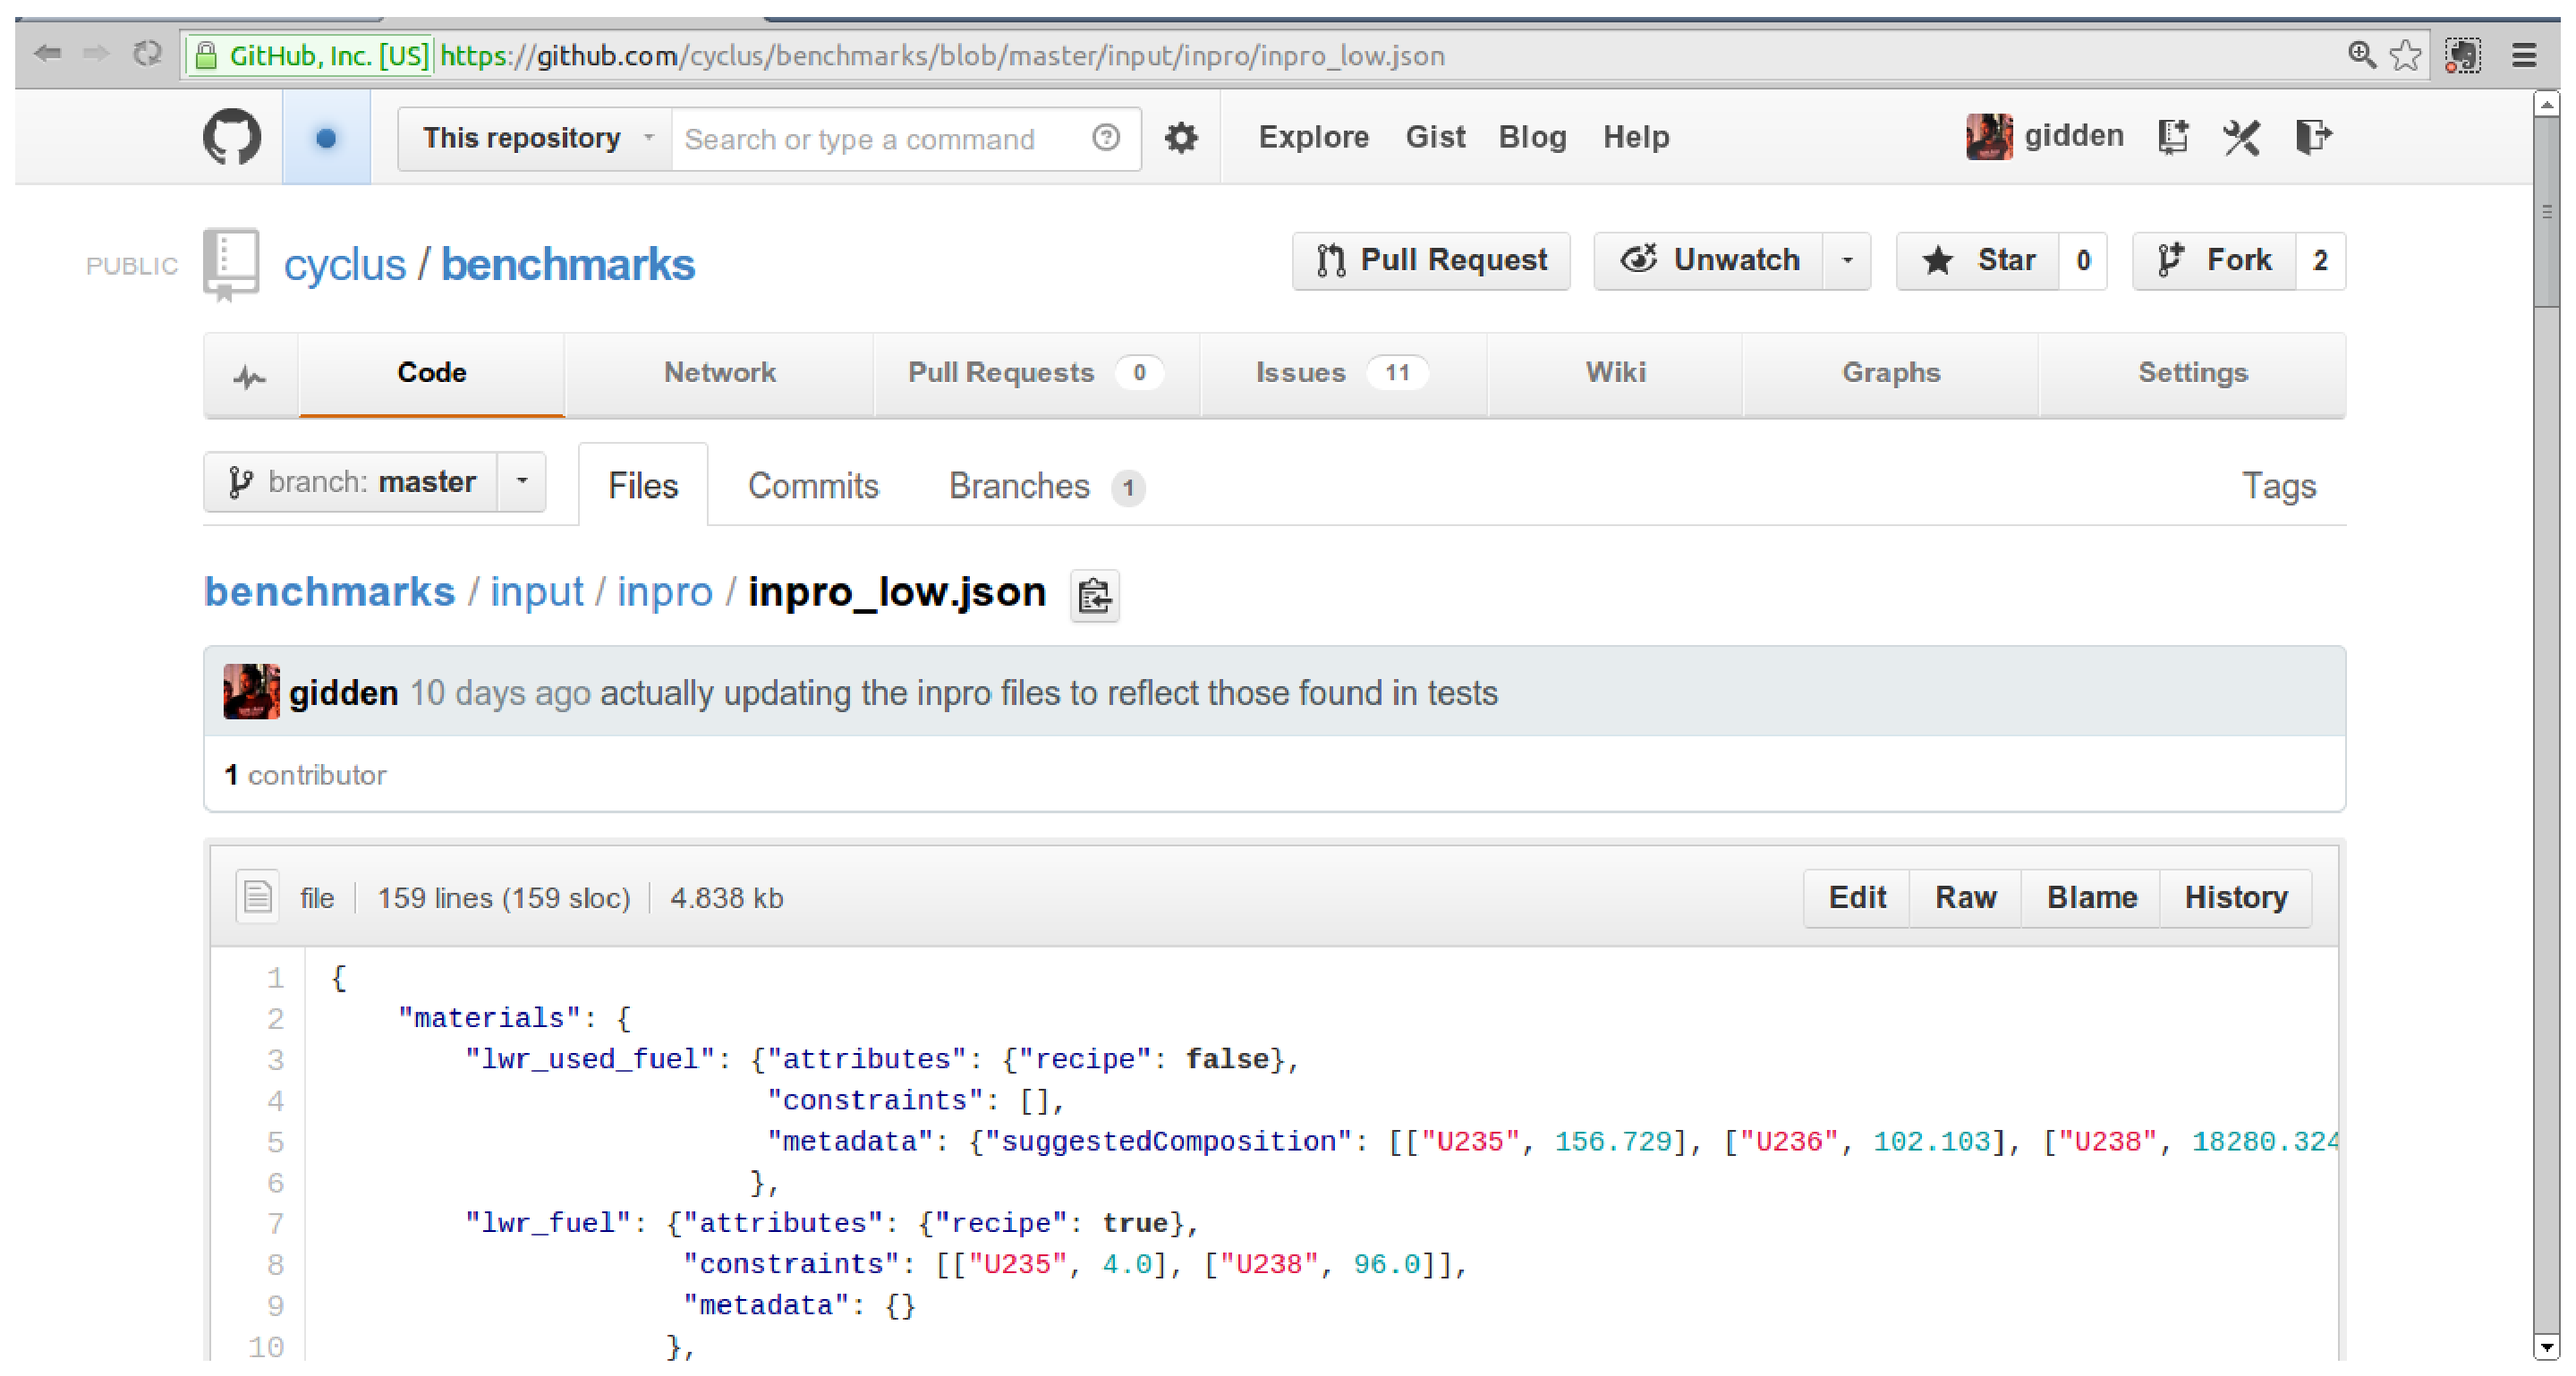
\includegraphics[width=\linewidth, height=\textheight, keepaspectratio]{inpro.eps}
    \caption{A Screenshot of the INPRO JSON File.}
  \end{figure}
\end{frame}

\begin{frame}
  \frametitle{Proposal : NEA Once Through}
  \begin{figure}
    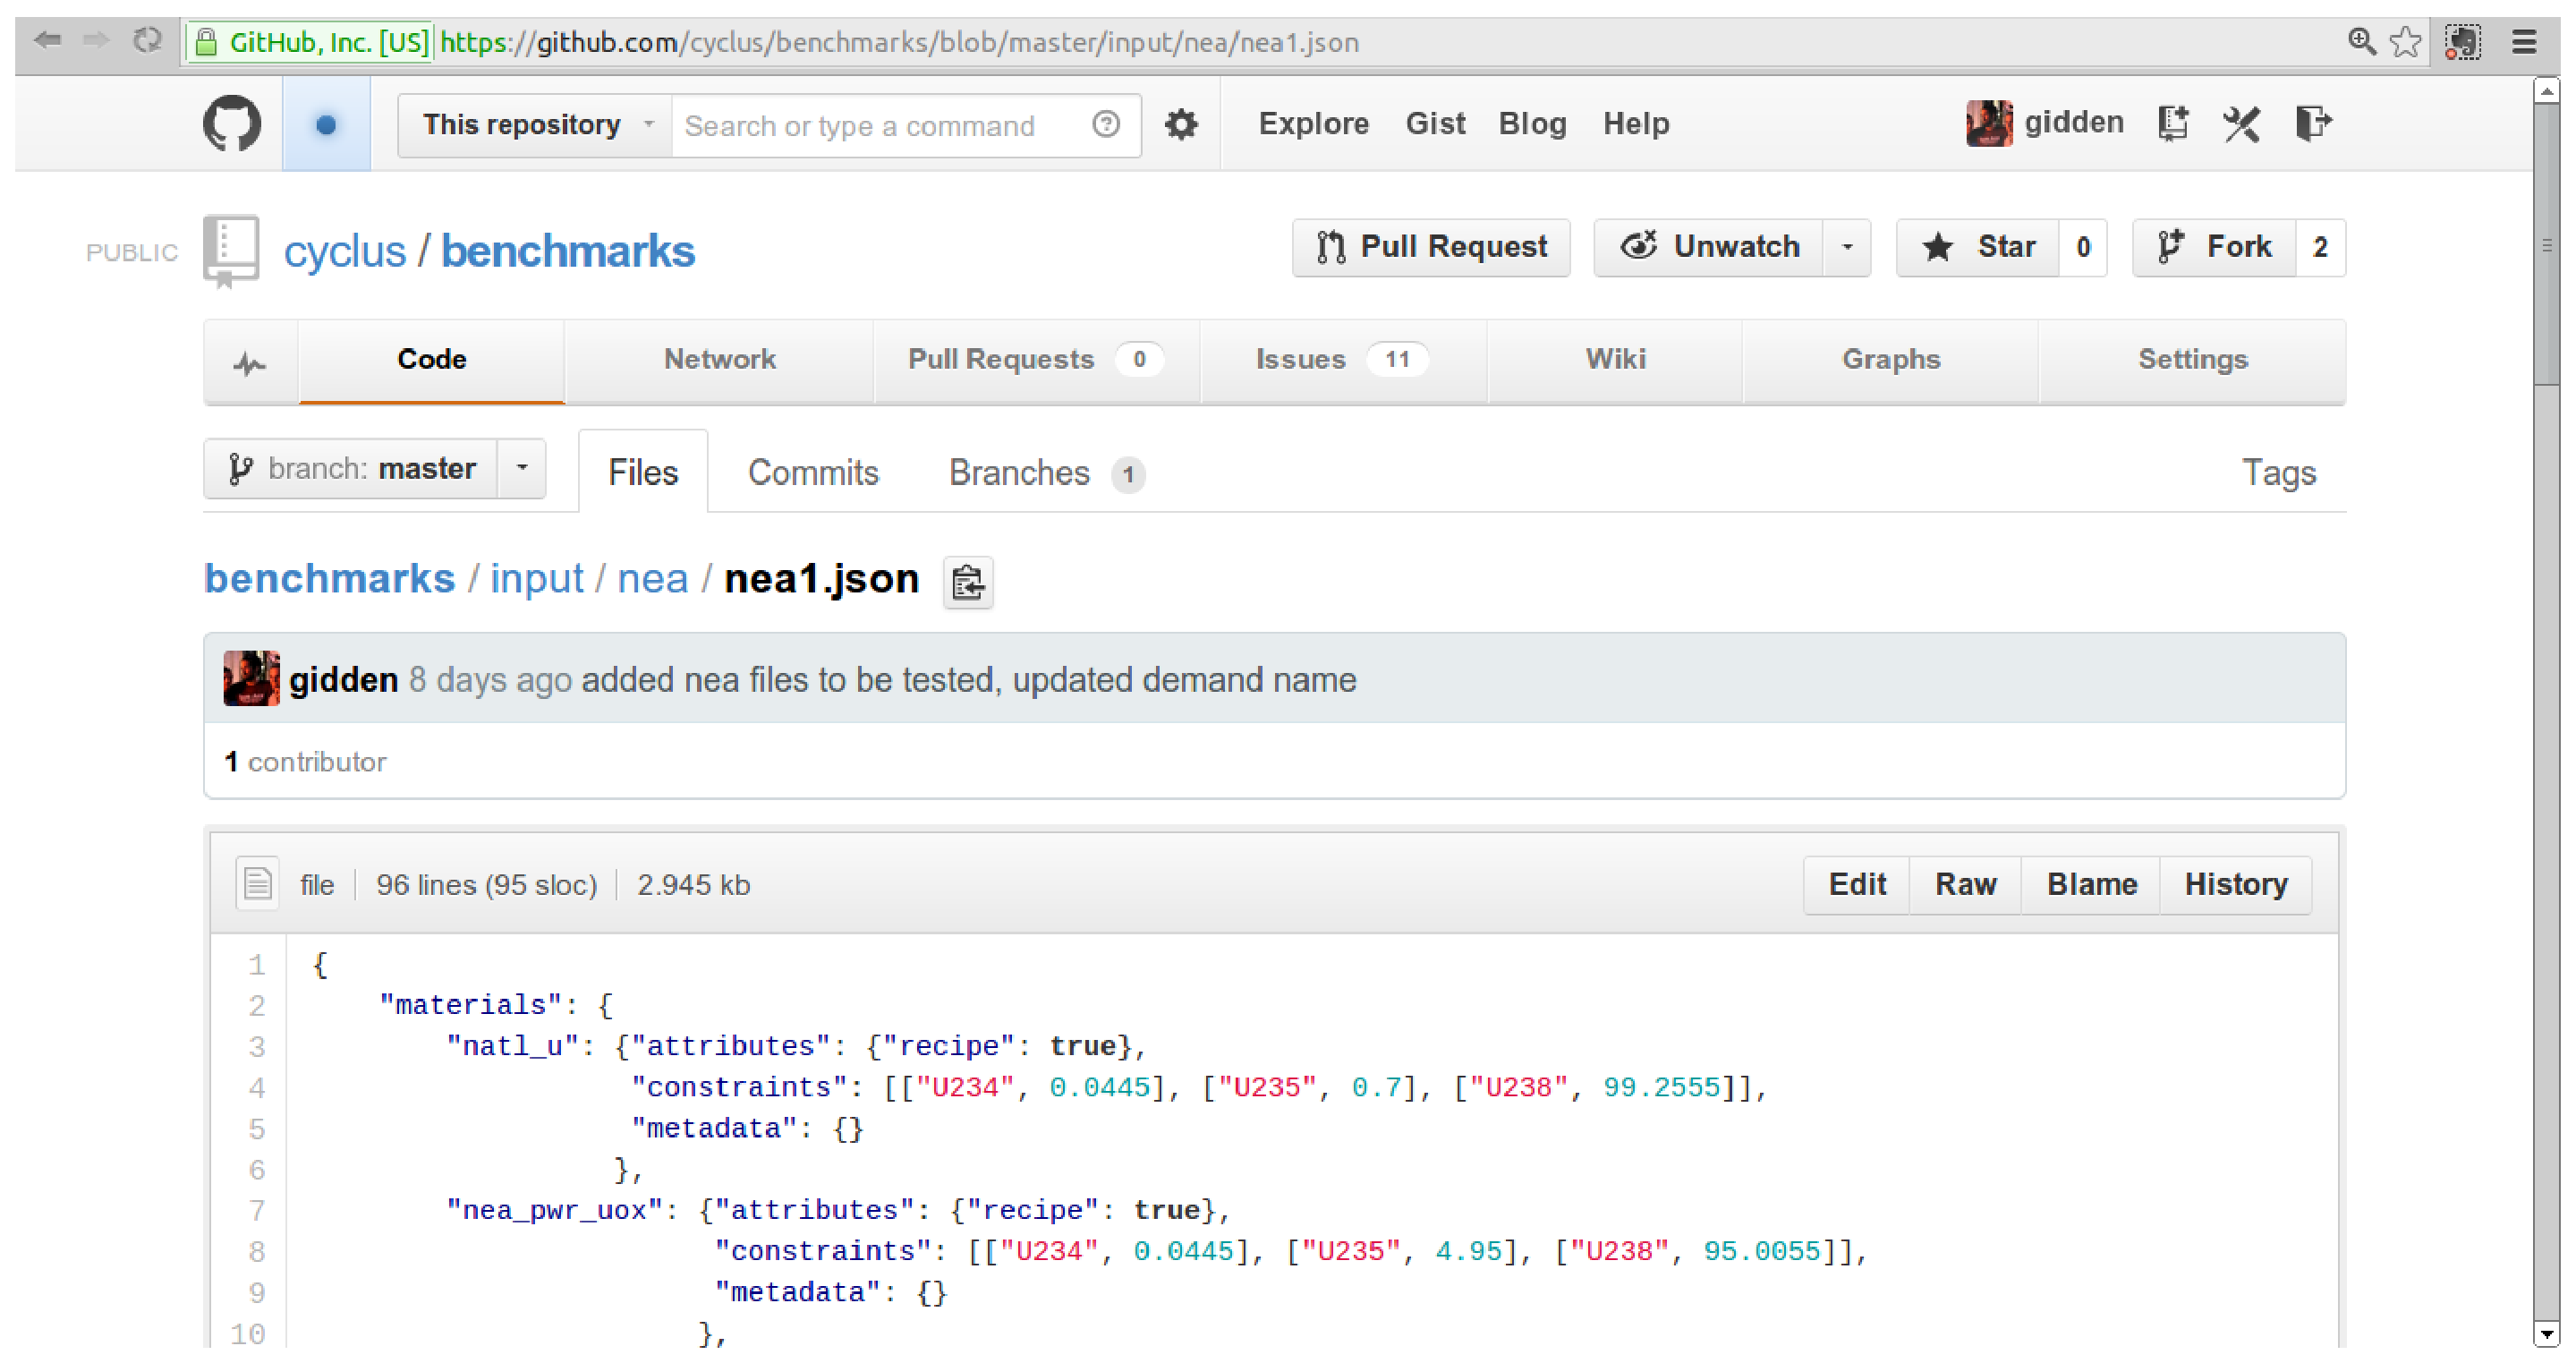
\includegraphics[width=\linewidth, height=\textheight, keepaspectratio]{nea.eps}
    \caption{A Screenshot of the NEA JSON File.}
  \end{figure}
\end{frame}

\begin{frame}
  \frametitle{Proposal : Translation} 
  With a common language specification, specific simulators can translate a
  specified benchmark.

  The Cyclus team has implemented one such option in Python.

  INPRO and NEA once-through benchmarks were translated, run in Cyclus, and
  compared with output, our previous benchmarking exercises.
\end{frame}

\begin{frame}[label = current]
  \frametitle{Proposal : Cyclus Translator}
  \begin{figure}
    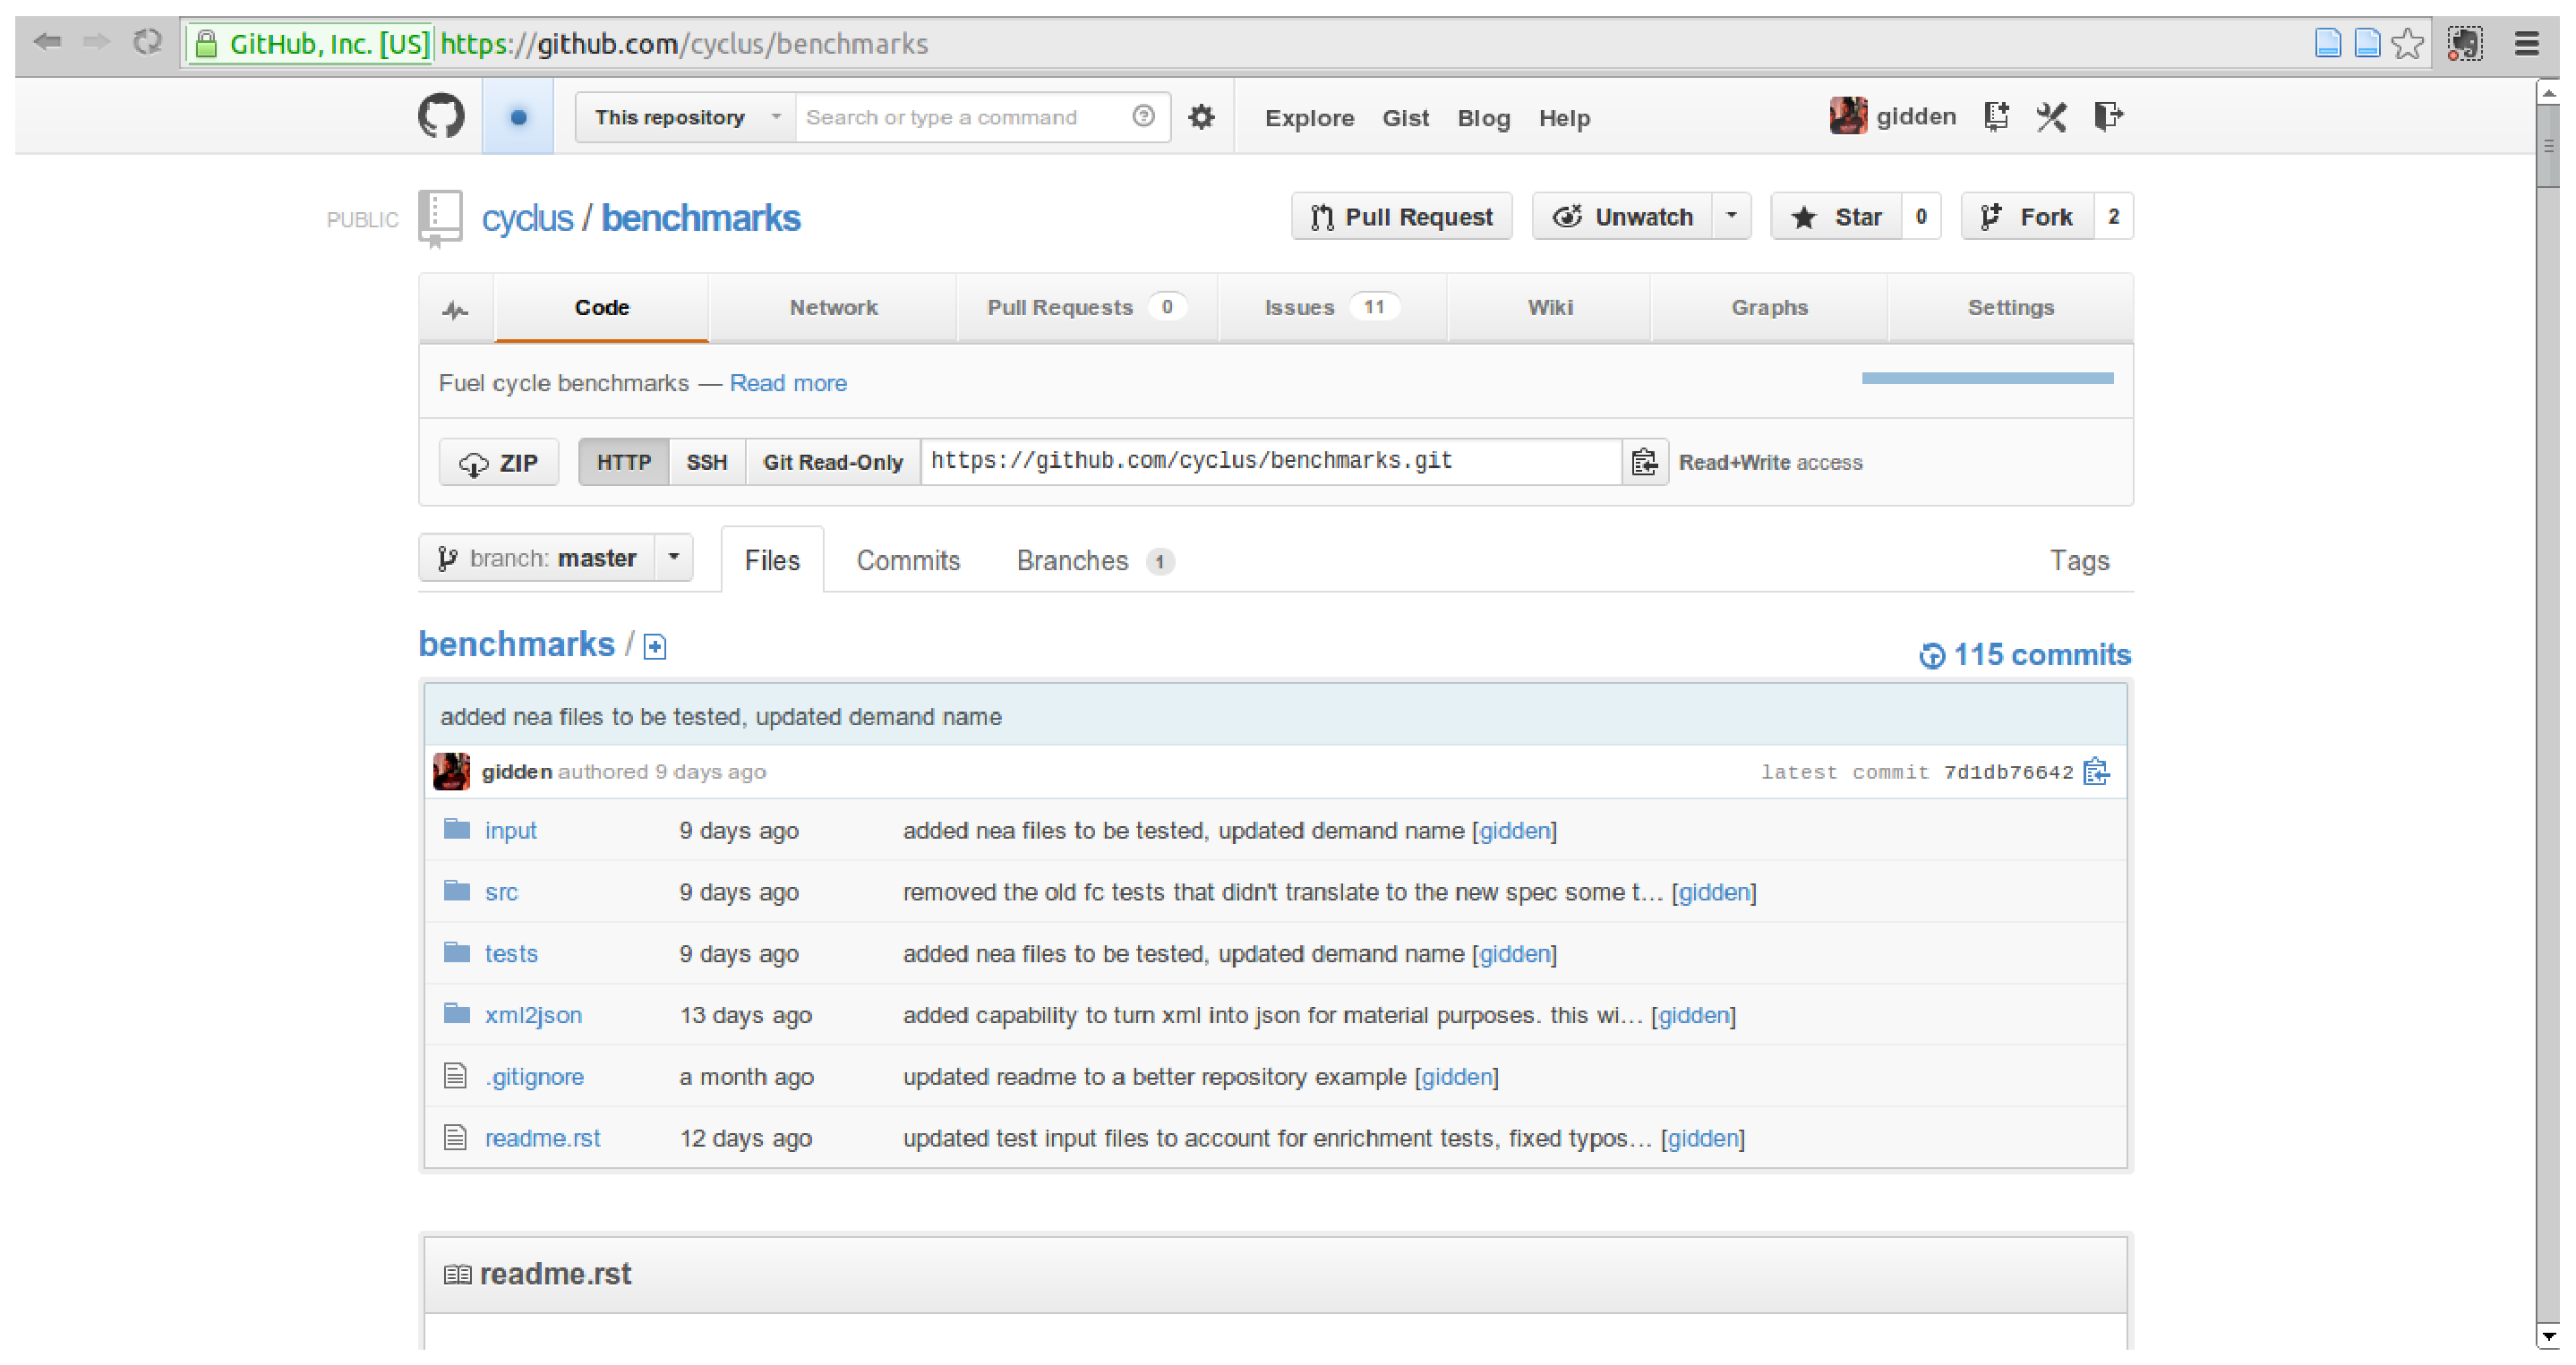
\includegraphics[width=\linewidth, height=\textheight, keepaspectratio]{benchmarks.eps}
    \caption{A Screenshot of the Cyclus Translator Repository.}
  \end{figure}
\end{frame}

\section{Conclusions}
% Overview : conclusions.tex

\begin{frame}
  \frametitle{Conclusions : Future Work}
  There's still lots to be done:
  \begin{itemize}
    \item Discuss with VISION team
    \item Profile existing code
    \item Add recycle capability
    \item Explore more fuel cycle option space
  \end{itemize}
  Cyclus is open source, feel free to join us!
\end{frame}

\section{Acknowledgements}
\begin{frame}[ctb!]
  \frametitle{Acknowledgments}
  First and foremost, I would like to thank the members of the
  Computational Nuclear Engineering Research Group at UW 
  \begin{itemize}
    \item Katy Huff
    \item Robert Carlsen
    \item Dr. Anthony Scopatz
    \item Dr. Paul Wilson
  \end{itemize}

  \vspace{0.2cm}

  And, of course, I would like to thank the DOE Office of Nuclear Energy's 
  Nuclear Engineering University Programs for providing funding. 
  \begin{figure}[htbp!]
    \begin{center}
      
\includegraphics[height=2cm]{neup.ps}
    \end{center}
    \label{fig:neup}
  \end{figure}
\end{frame}


%||||---------------
\begin{frame}[allowframebreaks]
  \frametitle{References}
  \bibliographystyle{plain}
  \bibliography{main}
\end{frame}
%---------------||||




\end{document}
